\documentclass[11pt,letterpaper]{article}
%% === margins ===
\addtolength{\hoffset}{-0.75in} \addtolength{\voffset}{-0.75in}
\addtolength{\textwidth}{1.5in} \addtolength{\textheight}{1.6in}
%% === basic packages ===
\usepackage{latexsym}
\usepackage{amssymb,amsmath}
\usepackage{graphicx}
\usepackage{booktabs}
%% === bibliography packages ===
\usepackage{apalike}
\bibliographystyle{apalike}
%% === hyperref options ===
\usepackage{color}
\usepackage[pdftex, bookmarksopen=true, bookmarksnumbered=true, 
pdfstartview=FitH, breaklinks=true, urlbordercolor={0 1 0}, citebordercolor={0 0 1}]{hyperref}  

% === dcolumn package ===
\usepackage{dcolumn}
\newcolumntype{.}{D{.}{.}{-1}}
\newcolumntype{d}[1]{D{.}{.}{#1}}
% === theorem package ===
\usepackage{theorem}
\theoremstyle{plain}
\theoremheaderfont{\scshape}
\newtheorem{proposition}{Proposition}
\newtheorem{assumption}{Assumption}
\def\qed{\hfill \vrule height7.5pt width6.17pt depth0pt}

% ==== rotating package ===
\usepackage{rotating}

% ==== dotted lines in tables ===
\usepackage{arydshln}

% == spacing between sections and subsections
\usepackage[compact]{titlesec} 

\begin{document}

% === new commands ===
\newcommand\ud{\mathrm{d}}
\newcommand\dist{\buildrel\rm d\over\sim}
\newcommand\ind{\stackrel{\rm indep.}{\sim}}
\newcommand\iid{\stackrel{\rm i.i.d.}{\sim}}
\newcommand\logit{{\rm logit}}
\renewcommand\r{\right}
\renewcommand\l{\left}
\newcommand\cA{\mathcal{A}}
\newcommand\spacingset[1]{\renewcommand{\baselinestretch}%
{#1}\small\normalsize}

\newcommand{\blind}{0} \newcommand{\tit}{eAppendix for ``Quantifying the Contribution of Earlier Detection and Advancements in Treatment on Gains in Life Expectancy for US Breast Cancer Patients Since 1975''}
%%%%%%%%%%%%%%%%%%%%%%%%%%%%%%%%%%%%%%%%%%%%%%%%%%%%%%%%%%%%%%%%%%%%%%%%

\if0\blind

 {\title{\bf \tit}
 
  \author{Samir Soneji\thanks{Dartmouth Institute for Health Policy \&
      Clinical Practice and Norris Cotton Cancer Center,
      Geisel School of Medicine at Dartmouth. Email: \href{mailto:samir.soneji@dartmouth.edu}{samir.soneji@dartmouth.edu}}
  \quad \quad 
  Hiram Beltr\'{a}n-S\'{a}nchez\thanks{Department of Community Health Sciences and California Center for Population Research, University of California, Los Angeles. Email:
    \href{mailto:beltrans@ucla.edu}{beltrans@ucla.edu}}}

\date{ }

\maketitle} \fi

% \begin{abstract}
% {\textbf{Background}.  US breast cancer mortality rates declined by 32\% since 1975, although the precise contributions of earlier detection and advancements in breast cancer treatment remain unknown.  We quantify the contributions of these two factors, as well as advancements in the treatment of other diseases, on gains in life expectancy among breast cancer patients.

% \textbf{Methods}.  We obtained annual incidence-based case fatality rates for 664,000 breast cancer patients aged 40 years and older from the Surveillance, Epidemiology, and End Results registries, 1975 to 2012.  We used life-table methods to calculate the gain in life expectancy and quantify the three constituent components of this gain: [1] earlier detection, [2] advancements in breast cancer treatment, and [3] advancements in the treatment of other diseases.  We additionally quantify which age groups contributed the most to the overall contribution of earlier detection.  We assumed a 10\% overdiagnosis level for tumors $\leq$3cm, and varied the level up to 32\% in a sensitivity analysis.

% \textbf{Results}.  Overall,  life expectancy increased 10.94 years between 1975 and 2002 for a 40-year old newly diagnosed breast cancer patient.  Advancements in breast cancer treatment contributed more to the gain in life expectancy than earlier detection: 6.79 years (62\%) versus 2.92 years (27\%).  Advancements in the treatment of other diseases contributed the remaining 1.25 years to this gain (11\%).  By age group, earlier detection among 40-49 year olds contributed more to the overall contribution of earlier detection (0.56 years) than 50-59 and 60-69 year olds (0.45 and 0.41 years, respectively).  We reached nearly identical substantive conclusions varying the level of overdiagnosis.

% \textbf{Conclusion}.  Life expectancy among breast cancer patients increased over time primarily because of advancements in breast cancer treatment, although the contribution of earlier detection was not trivial.}
% \end{abstract}
\if1\blind \title{\bf \tit} \maketitle \fi

\pdfbookmark[1]{Title Page}{Title Page}

\thispagestyle{empty}
\setcounter{page}{0}



\newpage
\clearpage
%%%%%%%%%%%%%%%%%%%%%%%%%%%%%%%%%%%%%%%%%%%%%%%%%%%%%%%%%%%%%%%%%%%%%%
 \setcounter{table}{0}  % reset counter for equation numbers
 \setcounter{figure}{0}  % reset counter for equation numbers
 \setcounter{page}{1}
 \renewcommand{\figurename}{Supplemental Figure}
 \renewcommand{\tablename}{Supplemental Table}
%\clearpage
%\pagenumbering{gobble}
\appendix

\spacingset{1.5}
\section{Computation of Incidence-Based Case Fatality Rates}
An incidence-based case fatality rate for a specific cohort of newly
diagnosed breast cancer patients equals the ratio of [1] the number of
deaths occurring for this cohort up to 10 years beyond their diagnosis
and [2] the total number of person-years lived by this cohort up to 10
years beyond their diagnosis.  For example, 556 women aged 65-69 years
were diagnosed with $<$1 cm breast cancer in 2001.  Between 2001 and
2011, 22 of these women died of breast cancer and another 107 died of
a competing cause of death.  This entire cohort lived a total of
5099.5 person-years over the 10-year period.  Thus, the
incidence-based case fatality rate from breast cancer equaled
22/5099.5 and the incidence-based case fatality rate from competing
causes of death equaled 107/5099.5.  Also, the proportion of women
diagnosed with $<$1cm breast cancer in 2001 equaled 4,602 out of 19,029
newly diagnosed breast cancers (24.2\%).

\section{Adjustment for Overdiagnosis}
Suppose 10\% of the 556 women aged 65-69 years old diagnosed with $<$1cm
breast cancer in 2001 were overdiagnosed, the observed case fatality
rate from breast cancer (22/5099.5) would become 22/[5099.5 -
0.10*5099.5].  Formally, let $\mathcal{A}$ be a set of starting ages
for age intervals analyzed (e.g., 40, 45, \dots, $\omega=100$ years), $\mathcal{T}$ be a set of
years (e.g., 1975, \dots 2002), and $\mathcal{S}$ be a set of tumor
sizes at diagnosis (e.g., $<$1cm, 1-2cm, 2-3cm, 3-5cm, and $\geq$5cm).
Let $\alpha_s$ represent the assumed level of overdiagnosis for tumor
size $s\in\mathcal{S}$.  Let $m_{a,t,s}$ represent the observed case
fatality rate for age group $a \in \mathcal{A}$, year $t \in
\mathcal{T}$, and tumor size $s \in \mathcal{S}$.  Then, the case
fatality rate adjusted for overdiagnosis equals:
\begin{eqnarray}
m^*_{a,t,s}=\frac{1}{1-\alpha_s} \times m_{a,t,s}. \notag
\end{eqnarray}

In 2001, the number of women diagnosed with breast cancer equaled:
4602 with $<$1cm tumors, 7208 with 1-2cm tumors, 3684 with 2-3cm
tumors, and 1300 with $\geq$5cm tumors.  These counts translate to the
following distribution: 24\%, 38\% 19\%, 12\%, and 7\%, respectively.
Suppose 10\% of $<$1cm breast cancers were overdiagnosed (460 of 4602
women).  We subtract these 460 women from the count of breast cancers
in 2001 and recalculate the distribution: 22\% for $<$1cm, 39\% for
1-2cm, 20\% for 2-3cm, 12\% for 3-5cm, and 7\% for $\geq$5cm.  
Let $\alpha_s$ represent the assumed level of overdiagnosis for tumor
size $s\in\mathcal{S}$.  Let $n_{t,s}$ represent the observed count
of breast cancer cases in year $t$ and for tumor size $s$.  The
observed distribution of incident breast cancer cases, $\pi_{t,s}$, equals
$\frac{n_{t,s}}{\sum_{s\in\mathcal{S}}n_{t,s}}$.  The distribution of
incident breast cancer cases adjusted for overdiagnosis equals: 
\begin{eqnarray}
\pi^*_{t,s}=\frac{(1-\alpha_s) \times n_{t,s}}{\sum_{s\in\mathcal{S}}
  (1-\alpha_s) \times n_{t,s}} \notag.
\end{eqnarray} 

\section{Computation of Tumor Size-Specific Life Expectancy}
The life expectancy of a breast cancer patient newly diagnosed at age
$a^*\in\mathcal{A}$, at time $t$, and with tumor size $s$ equals:
\begin{eqnarray}
 e_s(a^*,t)=\int_{a^*}^{\omega} e^{\left( -\int_{a*}^{a}\mu_s(y,t)\,dy \right)}da %=\int_{a^*}^{\omega} e^{\left(-\sum_{a=a*}^{a}n\,m^*_{a,t,s}\right)}\,da ,
\label{eq:ex.cont}
\end{eqnarray} 
where $\mu_s(a,t)$ %and $m^*_{a,t,s}$% 
represent the hazard of mortality
%and case fatality rate adjusted for overdiagnosis, respectively; $n$ is the width of the age interval; 
and $\omega$ is the starting age of
the final and open-ended age interval.

\subsection{Calculation of Life Expectancy from a Period Life Table}
\label{subsec:period_lifetable}
\spacingset{1.5} Although the theoretical definition of life
expectancy is given within the continuous-time framework, as shown in
Equation~(\ref{eq:ex.cont}), the data are typically recorded in a
discrete form.  A period life table is a common source of discrete
data, and is often analyzed in order to approximate the
continuous-time mortality process. Kitigawa and
Beltr\'{a}n-S\'{a}nchez decomposition methods both require the use of
a period life table. A main purpose of a period life table is to
calculate the life expectancy of a hypothetical cohort that
experiences the currently observed cross-sectional mortality rates.

Let $\cA$ be a set of the starting ages for the age intervals of a
period life table. We use $\omega$ to denote the starting age of the
oldest age interval. Let $n_x$ represent the width (years) of an age
interval starting at age $x \in \cA$. Typically, the width of age
intervals is the same for all but the youngest and oldest age intervals $[\omega,
\infty)$, e.g., $n_x=5$ for all $x \in \cA \setminus \{0,1,\omega\}$ and
$n_\omega=\infty$.  When $n_x>1$, a period life table is said to be
abridged.

A period life table is created by first observing the mid-interval
population, denoted by $_{n_x}P_x$, and the total number of deaths,
denoted by $_{n_x}D_x$, for each interval $[x,x+n_x)$.  Then, the
observed mortality rate for each interval, denoted by $_{n_x}M_x$, is
calculated as $_{n_x}D_x/_{n_x}P_x$.  Keeping with the standard
demographic notation, we use prescripts to indicate the width of the
interval under consideration.  A period life table relies on the
following stationarity assumptions of the population
\cite{chiang84,PreHeuGui00}:
\begin{enumerate}
\spacingset{1.0}
\item The age-specific hazard rate is constant over
  time, i.e., $\mu(x,t)=\mu(x)$ for all $t\in\mathcal{T}$;
\item The birth rate is constant over time; and
\item The net migration rates are zero at all ages.
\end{enumerate}

The assumptions imply that the survival function is also constant over
time, i.e., $l(x,y)=l(x)$, and that the crude death rate, i.e.,
$\sum_{x\; \in \cA} \,_{n_x}D_x/\sum_{x\; \in \cA}\,_{n_x}P_x$, equals
the crude birth rate, i.e., $B / \sum_{x\; \in \cA}\,_{n_x}P_x$, where
$B$ is the total number of births to members of the population in the
period.  Therefore, the total size of the hypothetical cohort is
assumed to remain constant over time. Another important consequence of
stationarity assumptions is that the age distribution of the
hypothetical cohort in any given interval, $[x,x+n_x)$, is constant
over time and is proportional to the survival function. Formally, for
all $s \in [x, x+n_x)$, the age distribution is defined by the
following density function,
\begin{eqnarray}
   \frac{l(s)}{\int_x^{x+n_x} l(t)\, dt},  
\label{eq:age}
\end{eqnarray}
A common departure from stationarity occurs in many
developing countries today, where annual births have been growing
relative to deaths. A violation of the stationarity assumptions is
also possible in developed countries where the death rates are
declining due to the advance of medical technologies.

Since $_{n_x}P_x$ and $_{n_x}D_x$ are directly obtained from the
Census data and vital statistics, they are typically large and
represent the total deaths and population of the country.  Thus, in
the literature, the sampling variability about the mortality rate of
the hypothetical cohort, denoted by $_{n_x}m_x$, is considered to be
small and hence typically ignored. That is, $_{n_x}M_x$ is assumed to
equal $_{n_x}m_x$, which is given by,
\begin{eqnarray}
  _{n_x}m_x & = & \frac{\int_x^{x+n_x} l(t) \mu(t)\, dt}{\int_x^{x+n_x}
    l(t)\, dt}, \label{eq:nmx}
\end{eqnarray}
for all $x \in \cA$.  

Furthermore, it can be shown that the conditional probability of death
within an interval $[x,x+n_x)$ given that an individual of the
hypothetical cohort survived up to age $x$, which is denoted by
$_{n_x}q_x$, is equal to
$n_x\;_{n_x}m_x/[1+(n_x-\,_{n_x}a_x)\,_{n_x}m_x]$, where $_{n_x}a_x$
represents the average person-years lived in a given interval $[x,
x+n)$ among those who are alive at age $x$ but die within the
interval.  The values of $_{n_x}a_x$ are obtained from complete life
tables and used in subsequent calculations as a known quantity
\cite{PreHeuGui00}.

Within this framework, the total number of person-years lived in an
interval, $[x, x+n_x)$, is given by,
\begin{eqnarray}
  _{n_x}L_x & = & n_x\,l_{x+n_x}\,+\,l_x\;_{n_x}q_x\;_{n_x}a_x,\label{eq:Lx}
\end{eqnarray}
where the members of the $l_{x+n_x}$ proportion who survive the entire
interval each contribute $n_x$ years, and the members of the
$l_x\;_{n_x}q_x$ proportion who die in the interval contribute
$_{n_x}a_x$ years, on average.  Finally, life expectancy at age $x$ is
equal to the total number of person-years for subsequent age
intervals,
\begin{eqnarray}
  e_x & = & \frac{1}{l_x} \sum_{i\, \in \cA_x}\; _{n_i}L_{i}, \label{eq:ex}
\end{eqnarray}
where $\cA_x = \{i \in \cA: \; x \le i\}$.  Under stationarity
assumptions for the unbounded last age interval $[\omega,\infty)$,
life expectancy at age $\omega$ is equal to the inverse of the death
rate, i.e., $e_\omega=\,_\infty m_\omega^{-1}$.  The equality follows
from the fact that all those alive at age $\omega$ must die in the
interval, i.e., $_\infty q_\omega=1$.

We now show that under stationarity assumptions discussed above,
$e_x$, which is the life expectancy calculated from a period life
table in Equation~(\ref{eq:ex}), equals $e(x)$, which is the
theoretical definition of life expectancy given in
Equation~(\ref{eq:ex.cont}).  Although in common demographic notation,
$l(x)$ is used in continuous notation and $l_x$ in discrete, both
refer to the proportion alive at exact age $x$ and hence are
numerically identical.  Given the hazard function, $\mu(x)$, the
conditional probability of death for an age interval, $[x,x+n_x)$, is
equal to the number of deaths in an age interval divided by the
proportion alive at the beginning of the age interval,
\begin{eqnarray}
  _{n_x}q_x & = & \frac{\int_x^{x+n_x} l(t)\,\mu(t)\,dt}{l(x)}. \label{eq:qx}
\end{eqnarray}
Next, the average number of years lived in an interval among those who
die in the interval is equal to the total number of person-years lived
among those who will die divided by the proportion who will die in the
interval,
\begin{eqnarray}
  _{n_x}a_x & = & \frac{\int_x^{x+n_x} l(t)\,\mu(t)\,(t-x)\,dt}
  {\int_x^{x+n_x}l(t)\,\mu(t)\,dt}. \label{eq:ax}
\end{eqnarray}
Substituting Equations~(\ref{eq:qx})~and~(\ref{eq:ax}) into
Equation~(\ref{eq:Lx}) and integrating it by parts yield,
\begin{eqnarray}
  _{n_x}L_x & = & \int_x^{x+n_x} l(t)\,dt. \label{eq:Lx_integral}
\end{eqnarray}  
Therefore, it follows that $e_x$ equals $e(x)$.

Table~\ref{tb:lifetable} shows the 1975 U.S. female abridged period
life table.  The radix, $l_0$, is set at $1$ so that $l_x$ represents
the survival probability.  From age $0$ to $\omega$,
the cohort will live
$\sum_{i=0}^{\omega}{_n}L_i=76.45$ person-years.  Hence, a $0$ year-old
member of the hypothetical cohort will live, on average, $76.45$ years
given she experiences these prevailing period age-specific
conditional probabilities of death.  For the last age group,
$_\infty a_{100}=e_{100}$ because everyone who is alive at age
$\omega=100$ dies within the last interval.

\begin{table}[htbp]
\spacingset{1}
\centering
\begin{tabular}{lrrrrrrrrr}
  \toprule
Age $x$ & $n_x$ & $_nm_x$ & $_nq_x$& $_na_x$ & $l_x$ & $_nd_x$ & $_nL_x$ & $T_x$ & $e_x$ \\ 
  \midrule
0 & 1 & 0.014 & 0.014 & 0.090 & 1.000 & 0.014 & 0.987 & 76.453 & 76.450 \\ 
  1 & 4 & 0.001 & 0.003 & 1.630 & 0.986 & 0.003 & 3.938 & 75.466 & 76.540 \\ 
  5 & 5 & 0.000 & 0.001 & 2.300 & 0.983 & 0.001 & 4.913 & 71.528 & 72.730 \\ 
  10 & 5 & 0.000 & 0.001 & 2.680 & 0.982 & 0.001 & 4.907 & 66.615 & 67.830 \\ 
  15 & 5 & 0.001 & 0.003 & 2.710 & 0.981 & 0.003 & 4.898 & 61.708 & 62.920 \\ 
  20 & 5 & 0.001 & 0.003 & 2.530 & 0.978 & 0.003 & 4.883 & 56.810 & 58.080 \\ 
  25 & 5 & 0.001 & 0.004 & 2.580 & 0.975 & 0.004 & 4.866 & 51.927 & 53.260 \\ 
  30 & 5 & 0.001 & 0.005 & 2.600 & 0.971 & 0.005 & 4.846 & 47.061 & 48.450 \\ 
  35 & 5 & 0.001 & 0.007 & 2.680 & 0.967 & 0.007 & 4.817 & 42.215 & 43.670 \\ 
  40 & 5 & 0.002 & 0.012 & 2.660 & 0.960 & 0.011 & 4.772 & 37.398 & 38.970 \\ 
  45 & 5 & 0.004 & 0.018 & 2.670 & 0.948 & 0.017 & 4.701 & 32.627 & 34.410 \\ 
  50 & 5 & 0.005 & 0.027 & 2.640 & 0.931 & 0.025 & 4.597 & 27.925 & 29.990 \\ 
  55 & 5 & 0.008 & 0.040 & 2.650 & 0.906 & 0.036 & 4.446 & 23.328 & 25.740 \\ 
  60 & 5 & 0.012 & 0.058 & 2.610 & 0.870 & 0.051 & 4.229 & 18.882 & 21.700 \\ 
  65 & 5 & 0.017 & 0.083 & 2.650 & 0.819 & 0.068 & 3.936 & 14.653 & 17.880 \\ 
  70 & 5 & 0.029 & 0.138 & 2.640 & 0.751 & 0.103 & 3.511 & 10.717 & 14.270 \\ 
  75 & 5 & 0.046 & 0.207 & 2.600 & 0.648 & 0.134 & 2.916 & 7.206 & 11.130 \\ 
  80 & 5 & 0.077 & 0.323 & 2.550 & 0.514 & 0.166 & 2.162 & 4.290 & 8.350 \\ 
  85 & 5 & 0.125 & 0.473 & 2.430 & 0.348 & 0.165 & 1.316 & 2.128 & 6.120 \\ 
  90 & 5 & 0.196 & 0.638 & 2.270 & 0.183 & 0.117 & 0.597 & 0.812 & 4.430 \\ 
  95 & 5 & 0.287 & 0.780 & 2.070 & 0.066 & 0.052 & 0.180 & 0.215 & 3.250 \\ 
  $\geq100$ & $\infty$ & 0.403 & 1.000 & 2.482 & 0.016 & 0.015 & 0.035 & 0.035 & 2.482 \\ 
   \bottomrule
\end{tabular}
\caption{The 1975 U.S. Female Period Life Table and Life Expectancy.  
  The period life table is created from the conditional
  probability of death, $_nq_x$, and the average person-years lived
  in the age interval by those dying in the interval, $_na_x$.
  $l_x$ is the proportion of survivors at age $x$, whereas $L_x$
  represents the total number of person-years lived within the age
  interval $[x, x+n_x)$ for those who were alive at age $x$. The
  last age interval is $[100, \infty)$. The final column gives the
  life expectancy $e_x$ at each age.}
    \label{tb:lifetable}
\end{table}

\spacingset{1.5}
\section{Schematic Representation of the Methodology}
For simplicity, consider three mutually exclusive and exhaustive
categories of tumor size: 1, 2, and 3 (e.g., $<$1cm, 1-2cm, and
$\geq$2cm).  Suppose the distribution of tumor size at cancer
diagnosis remained constant between times 1 and 2 (Supplemental
Figure~\ref{fig:simple_case}, Panel A), tumor size-specific case
fatality rates from breast cancer decreased between times 1 and 2
(Supplemental Figure~\ref{fig:simple_case}, Panel B), and tumor
size-specific case fatality rates from competing causes of death
remained constant between times 1 and 2 (Supplemental
Figure~\ref{fig:simple_case}, Panel B).  Tumor size-specific life
expectancy increased between times 1 and 2 because tumor size-specific
case fatality rates from breast cancer decreased over the time period
(Supplemental Figure~\ref{fig:simple_case}, Panel C).  Overall life
expectancy at each time equals the weighted average of tumor
size-specific life expectancy, where the weights equal the
distribution of tumor sizes at cancer diagnosis at times 1 and 2,
respectively.  Overall life expectancy grew between times 1 and 2, and
this gain was entirely due to decreases in tumor size-specific case
fatality rates from breast cancer (Supplemental
Figure~\ref{fig:simple_case}, Panel D).  In actuality, all three
aforementioned factors change over time and contribute to the gain in
life expectancy.  We quantify the individual contribution of each of
these three constituent components.  We also utilize the same
demographic method to further disaggregate these three contributions
by age group in Section~\ref{sec:age}.
\begin{figure}[h]
\begin{center}
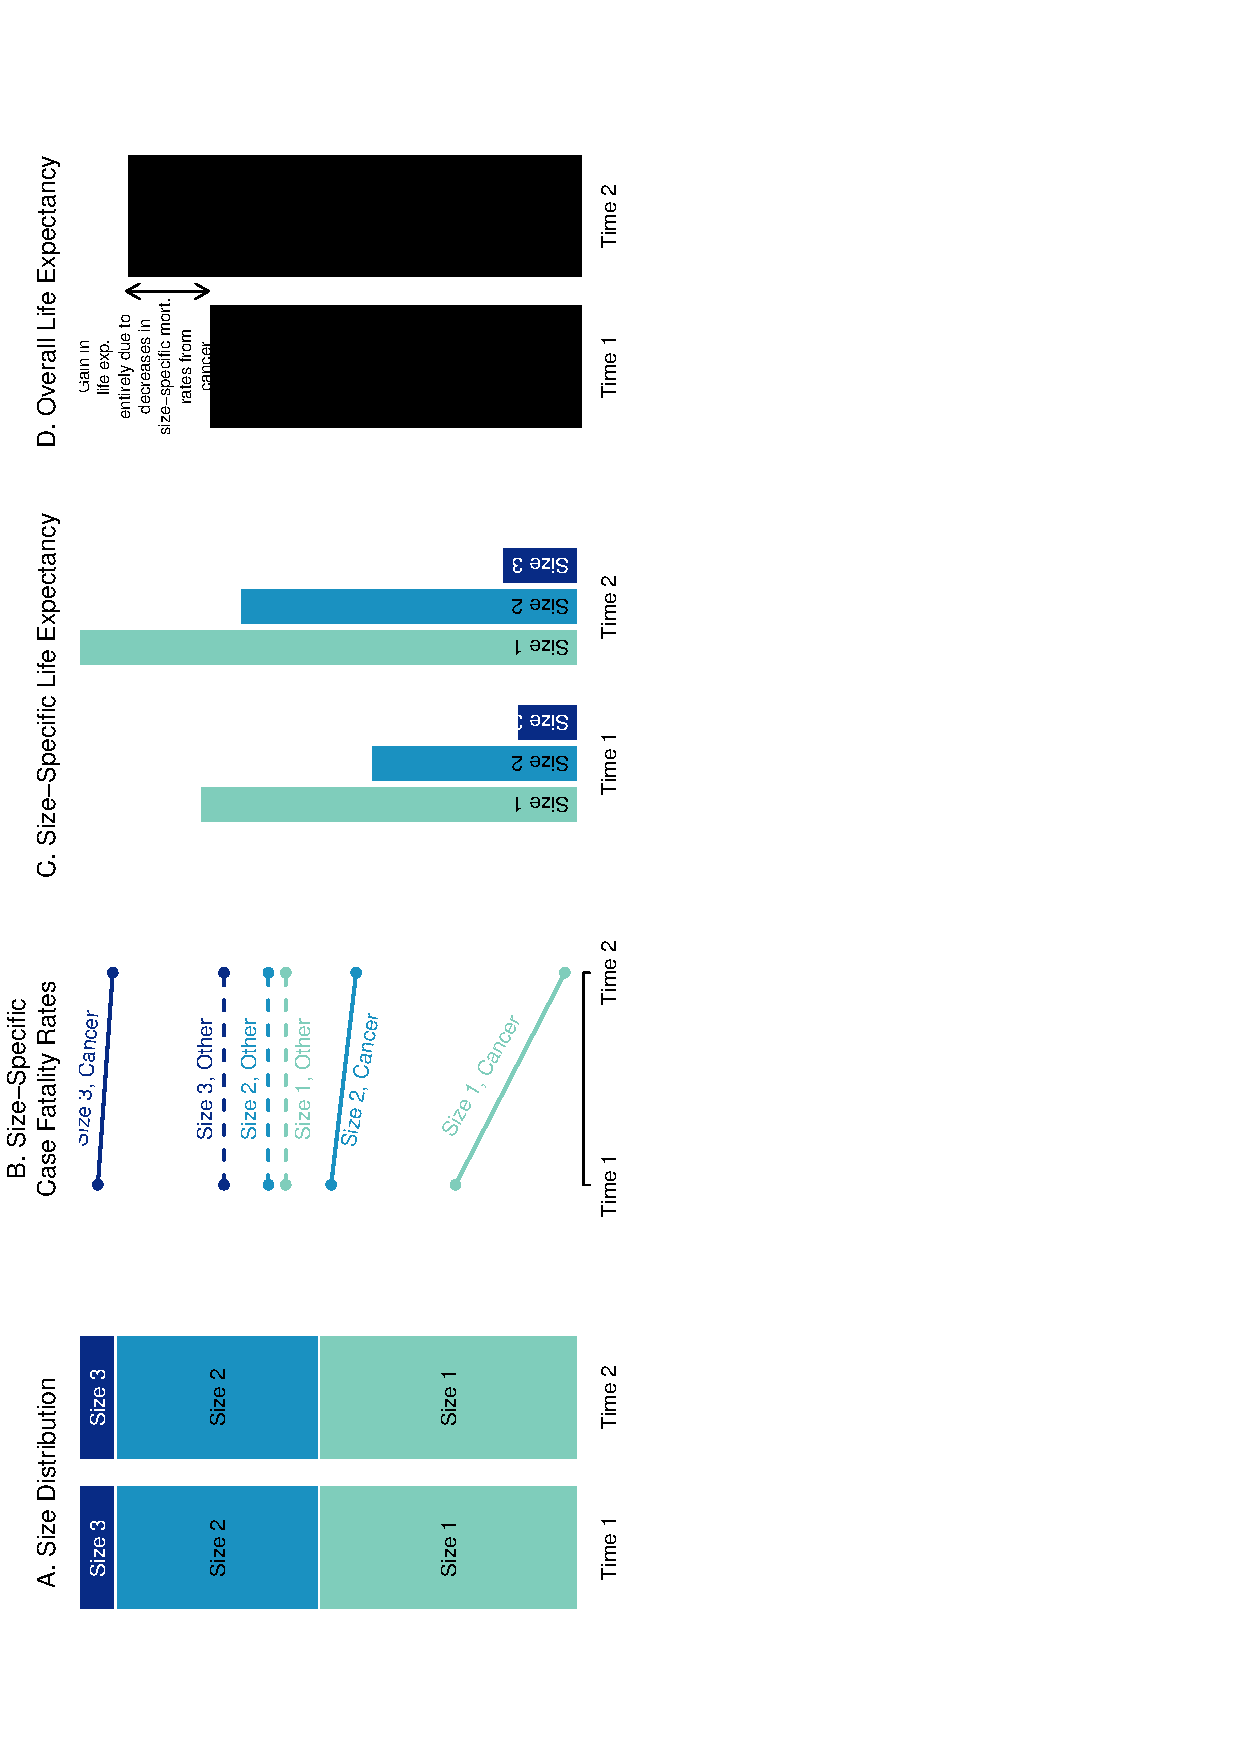
\includegraphics[trim=0 220 0 0,clip,width=\linewidth]{appendix_figure1}
\spacingset{1}\caption{The gain in life expectancy depends
  on three factors: (A) changes in the tumor size distribution at
  cancer diagnosis, (B) changes in tumor size-specific case fatality rates from
  breast cancer, and (C) changes in tumor size-specific case fatality rates from
  competing causes of death.}
\label{fig:simple_case}
\end{center}
\end{figure}

\section{Decomposition by Tumor Size and Case Fatality Rates from
  Breast Cancer and Other Causes of Death}
Let $\pi_s(t)$ equal the proportion of breast cancer patients
diagnosed with tumor size $s$ in year $t$.  Let $e_s(a,t)$ equal the
tumor size-specific life expectancy at age $a$. The overall life
expectancy at age $a$ and time $t$, $e(a,t)$, equals:
\begin{eqnarray}
  e(a,t)=\sum_{s\in\mathcal{S}}\,\pi_s(t)\,e_s(a,t), \notag
\end{eqnarray}
where $\sum_{s\in\mathcal{S}}\,\pi_s=1$. 

The change in life expectancy at age $a$ between times $t_1$ and $t_2$
can be decomposed using the methodology of \cite{Kitagawa55}:
\begin{align}
  e(a,t_2)-e(a,t_1)&=\sum_{s\in\mathcal{S}}\left[\,\pi_s(t_2)\,e_s(a,t_2)- \pi_s(t_1)\,e_s(a,t_1)\right]  \notag\\
  \hspace{-0.7in} &=\sum_{s\in\mathcal{S}}\left[\pi_s(t_2)-\pi_s(t_1)
  \right]\left[\frac{e_s(a,t_1)+e_s(a,t_2)}{2}\right]+ \notag\\
  &\phantom{=}\sum_{s\in\mathcal{S}}\left[e_s(a,t_2)-e_s(a,t_1)
  \right]\left[\frac{\pi_s(t_1)+\pi_s(t_2)}{2}\right].
 \label{eqn:decomp.basic}
\end{align}
 
Equation~(\ref{eqn:decomp.basic}) quantifies how much of the change in life
expectancy at age $a$ between times $t_1$ and $t_2$ is due to: [a]
shifts in the share of cancer tumor size (first term) and [b] changes
in tumor-size-specific life expectancy (second term).

We can further decompose the second term of
equation~\ref{eqn:decomp.basic} by cause of death. In doing so, we can
quantify how much of this change in tumor-size-specific cancer life
expectancy, $e_s(a,t_2)-e_s(a,t_1)$, is due to improvements in case
fatality rates from breast cancer and improvements in case fatality
rates from  competing causes of death.  Let $\mathcal{C}$ be a set of
mutually exclusive and exhaustive causes of death (e.g., breast cancer
and all other causes).  Let $L_{a,s,c}(t)$ represent the person-years
lived in the life table based on the case fatality rate at age $a$,
for tumor size $s$, from cause $c\in\mathcal{C}$, and at time $t$.
Similarly, let $L_{a,s,-c}(t)$ represent the person-years lived in the
life table based on the case fatality rate at age $a$, for tumor size
$s$, and from causes other than $c$ ($-c$), and at time $t$.  Let $a^*$ be
the first starting age of $\mathcal{A}$.  Then, following the approach
developed by \cite{BelPreCan08},
\begin{eqnarray}
e_s(a^*,t_2)-e_s(a^*,t_1)= \sum_{c\in\mathcal{C}}\sum_{a=a^*}^\omega \left[L_{a,s,c}(t_2)-L_{a,s,c}(t_1) \right] \left[\frac{L_{a,s,-c}(t_2)+L_{a,s,-c}(t_1) }{2n} \right],
\label{eqn:causedecomp}
\end{eqnarray}
where $n$ is the width of the age interval and $\omega$ is the
starting age of the final and open-ended age interval.

We perform the decomposition starting at age 40; the final
decomposition equation equals:
\begin{align*}
  e(40,t_2)-e(40,t_1)&=\sum_{s\in\mathcal{S}}\left[\,\pi_s(t_2)\,e_s(40,t_2)- \pi_s(t_1)\,e_s(40,t_1)\right] \notag \\
                     &=\sum_{s\in\mathcal{S}}\left[\pi_s(t_2)-\pi_s(t_1) \right]\left[\frac{e_s(40,t_1)+e_s(40,t_2)}{2}\right]+\sum_{s\in\mathcal{S}}\left[\mathtt{Diff_e} \right]\left[\frac{\pi_s(t_1)+\pi_s(t_2)}{2}\right],
\end{align*}
where $\mathtt{Diff_e}$ is given by equation \eqref{eqn:causedecomp} evaluated at $a^*=40$.\\


\section{Decomposition by Tumor Size, Case Fatality Rates from
  Breast Cancer and Other Causes of Death, and Age Group}
\label{sec:age}
As previously defined $\pi_{s}(t)$ equals the proportion of cancer patients with tumor size
$s$ in year $t$. This proportion can also be computed by age group
such that $\pi_s(t)=\sum_{a\in\mathcal{A}}\pi_{s,a}(t)$ and
$\sum_{s\in\mathcal{S}}\,\pi_s=1$.  Then, the
change in life expectancy at age $a$ between times $t_1$ and $t_2$ can
be estimated as:
\begin{align*}
  e(40,t_2)-e(40,t_1)&=\sum_{s\in\mathcal{S}}\left[\,\pi_s(t_2)\,e_s(40,t_2)- \pi_s(t_1)\,e_s(40,t_1)\right] \\
                     &=\sum_{s\in\mathcal{S}} \left[\sum_{a\in\mathcal{A}}\pi_{s,a}(t_2)\,e_s(40,t_2)- \sum_{a\in\mathcal{A}}\pi_{s,a}(t_1)\,e_s(40,t_1) \right]\\
                     &=\sum_{s\in\mathcal{S}}\left[\pi_{s,40}(t_2)\,e_s(40,t_2)-
                       \pi_{s,40}(t_1)\,e_s(40,t_1)\right] +\\
                     &\hspace{0.18in}\sum_{s\in\mathcal{S}}\left[\pi_{s,45}(t_2)\,e_s(40,t_2)- \pi_{s,45}(t_1)\,e_s(40,t_1)\right] + \\
  &\phantom{=\Sigma}\vdots \\
                     &\hspace{0.18in}\sum_{s\in\mathcal{S}}\left[\pi_{s,\omega}(t_2)\,e_s(40,t_{\omega})- \pi_{s,\omega}(t_1)\,e_s(40,t_1)\right]. \notag 
 \end{align*}


 Each summation in the above equation can be written as follows based
 on equation \eqref{eqn:decomp.basic}:
\begin{multline}
  e(40,t_2)-e(40,t_1)= \\
  \sum_{s\in\mathcal{S}}\left[\pi_{s,40}(t_2)-\pi_{s,40}(t_1) \right]\left[\frac{e_s(40,t_1)+e_s(40,t_2)}{2}\right]+\sum_{s\in\mathcal{S}}\left[e_s(40,t_2)-e_s(40,t_1) \right]\left[\frac{\pi_{s,40}(t_1)+\pi_{s,40}(t_2)}{2}\right] +\\
  \sum_{s\in\mathcal{S}}\left[\pi_{s,45}(t_2)-\pi_{s,45}(t_1) \right]\left[\frac{e_s(40,t_1)+e_s(40,t_2)}{2}\right]+\sum_{s\in\mathcal{S}}\left[e_s(40,t_2)-e_s(40,t_1) \right]\left[\frac{\pi_{s,45}(t_1)+\pi_{s,45}(t_2)}{2}\right] +\\
  \vdots \\
  \sum_{s\in\mathcal{S}}\left[\pi_{s,{\omega}}(t_2)-\pi_{s,{\omega}}(t_1) \right]\left[\frac{e_s(40,t_1)+e_s(40,t_2)}{2}\right]+\sum_{s\in\mathcal{S}}\left[e_s(40,t_2)-e_s(40,t_1) \right]\left[\frac{\pi_{s,{\omega}}(t_1)+\pi_{s,{\omega}}(t_2)}{2}\right] =\\
  \sum_{s\in\mathcal{S}}\left[\mathtt{Diff_{\pi,40}} \right]\mathtt{\bar{e}_s} + \sum_{s\in\mathcal{S}}\left[\mathtt{Diff_{\pi,45}} \right]\mathtt{\bar{e}_s} + 
  \dots +
 \sum_{s\in\mathcal{S}}\left[\mathtt{Diff_{\pi,{\omega}}} \right]\mathtt{\bar{e}_s} +\sum_{s\in\mathcal{S}}\left[e_s(40,t_2)-e_s(40,t_1)\right]\left[\frac{\pi_s(t_1)+\pi_s(t_2)}{2}\right]
\label{agedec}
\end{multline}
where $\mathtt{Diff_{\pi,a}}=\pi_{s,a}(t_2)-\pi_{s,a}(t_1)$ and $\mathtt{\bar{e}_i}=\frac{e_s(40,t_1)+e_s(40,t_2)}{2}$.

The terms of equation\eqref{agedec} that include
$\mathtt{Diff_{\pi,40}}\dots \mathtt{Diff_{\pi,\omega}}$ correspond to
the contribution of changes in the share of tumor size by age group to
the change in cancer life expectancy between times $t_1$ and $t_2$.
We can additionally estimate the contribution of changes in case
fatality rates from breast cancer and competing causes of death to
changes in tumor-size-specific life expectancy by age. The last term
of equation \eqref{agedec} can be written as follows, based on equation
\eqref{eqn:causedecomp}:
\begin{align}
  e_s(40,t_2)-e_s(40,t_1)&=\sum_{c\in\mathcal{C}} \sum_{a=40}^\omega\left[L_{a,s,c}(t_2)-L_{a,s,c}(t_1) \right] \left[\frac{L_{a,s,-c}(t_2)+L_{a,s,-c}(t_1) }{2n} \right].  
\end{align}

\section{Assuming Constant Mortality Within Age Intervals}
Let $M_{a,a+n}$ represent the mortality rate between ages $a$ and
$a+n$ and let $\mu(a)$ represent the hazard of mortality at age
$a$.  The number (or proportion) of survivors at age $a+n$ in the
life table, $l_{a+n}$, equals \cite{PreHeuGui00}:
\begin{equation}
l_{a+n}=l_{a}\,e^{-\int_a^{a+n}\mu(x)\,dx}=l_{a}\,e^{-n\,M_{a,a+n}}.\notag
\end{equation}
Then, the number of person-years lived between ages $a$ and $a+n$ equals:
\begin{equation}
_nL_{a}=l_a\,\int_a^{a+n} e^{-M_{a,a+n}(s-a)} ds=l_a \left(\frac{-1}{M_{a,a+n}}(e^{-n\,M_{a,a+n}}-1) \right).
\label{constant.Lx}
\end{equation}
Suppose the age interval is $n=5$ years wide, then equation \eqref{constant.Lx}
equals:
\begin{equation}
_5L_{a}=l_a \left(\frac{-1}{M_{a,a+5}}(e^{-5\,M_{a,a+5}}-1) \right).\notag
\end{equation}
For the last and open-ended age group (e.g., $\geq$100 years), we can assume there
are no person-years lived beyond a certain time (say no more than 10
years) to compute $_{\infty}L_{100}$ as:
\begin{equation}
_{\infty}L_{100}=l_{100} \left(\frac{-1}{M_{100+}}(e^{-10\,M_{100+}}-1) \right).\notag
\end{equation}

\newpage
\section{Varying Assumed Prevalence of Overdiagnosis for $<$1cm and $1-3$cm Tumors}
We individually varied the assumed prevalence of overdiagnosis from
0\% to 97\% for tumors $<$1cm and from 0\% to 52\% for 1-3cm tumors.
We set the upper bound based on the smallest percentage of SEER
patients diagnosed with $<$1cm tumors who subsequently died of breast
cancer within 10 years (3\%).  At conservative assumed
prevalences of overdiagnosis: 97\% for $<$1cm tumors and 35\% for
1-3cm tumors, the contribution to the 7.58-year gain in life
expectancy were: 6.40 years from reductions in case fatality rates
from breast cancer (84\%), 0.22 years from the temporal shift to
smaller sized tumors (3\%), and 0.98 years from reductions in case
fatality rates from competing causes of death (13\%).

\begin{figure}[h]
\begin{center}
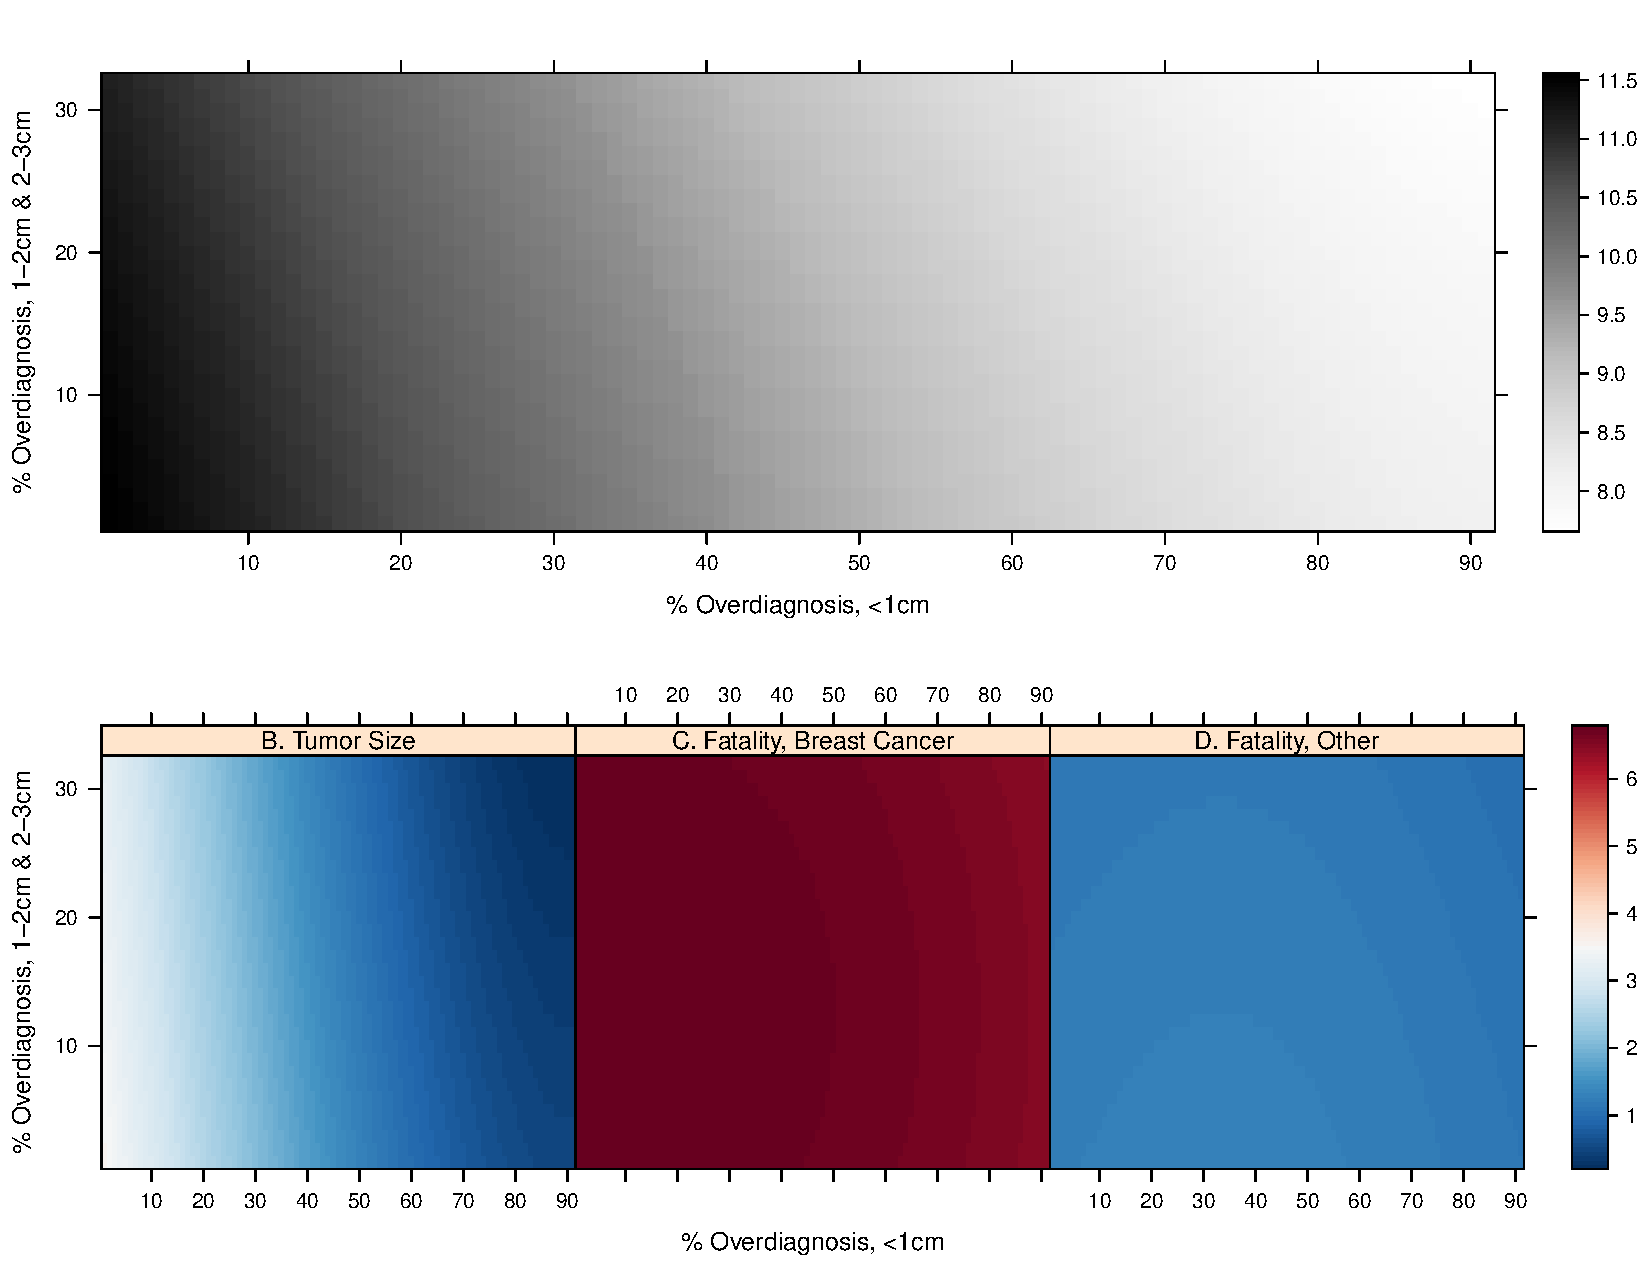
\includegraphics[scale=0.52]{appendix_figure2}
\spacingset{1}\caption{Gain in life expectancy (top panel) and
  contributions of the temporal shift to smaller sized tumors (bottom
  left), temporal reductions in case fatality rates from breast cancer
  (bottom center), and temporal reductions in case fatality rates from
  competing causes of death (bottom right) varying the overdiagnosis
  level for $<$1cm tumors (0\% to 90\%) and 1-3cm tumors (0\% to
  31\%).  The color scale for the top (bottom) panel indicates the
number of years of the gain in life expectancy (contribution to the gain).}
\label{fig:figure2}
\end{center}
\end{figure}

\newpage
\section{Bias in Life Expectancy and Gain in
  Life Expectancy Under CISNET Approach}
\spacingset{1.5} CISNET first estimates age- and time-specific mortality
rates from all other causes by subtracting breast cancer mortality
rates from all-cause mortality rates.  CISNET then generates an age of
death from all other causes by randomly drawing from the the age of
death distribution based on a set of the estimated mortality rates
from all other causes of death.  Second, CISNET generates an age of
death from breast cancer following screen detection based on the
patient's age and stage of detection.  Finally, CISNET sets the
overall age of death as the minimum of the age of death from all other
causes and the age of death from breast cancer.  We show below that the
CISNET approach yields biased estimates of life expectancy and the
gain in life expectancy.

\subsection{Mathematical Proof of Bias}
In this section, we prove mathematically that the CISNET approach
yields biased estimates of life expectancy and the gain in life
expectancy.  Let $X$ be a continuous random variable that represents the
age of death when the only cause of death is breast cancer.  Let $Y$ be
a continuous random variable that represents the age of death when the
only cause of death is all other causes.  And let $Z$ be a continuous
random variable that represents the age of death for all causes of
death.

First, $\text{min}(X,Y) \leq X$.  By the linearity of expectation,
$E[\text{min}(X,Y)] \leq E(X)$,  Similarly, $\text{min}(X,Y) \leq Y$ and
$E[\text{min}(X,Y)] \leq E(Y)$.  Then, 
\begin{eqnarray}
E[\text{min}(X,Y)] \leq \text{min}[E(X),E(Y)]. 
\label{eq:min.xy}
\end{eqnarray}
 The left term of equation~(\ref{eq:min.xy}) represents the estimate of
 life expectancy under the CISNET approach.  

Consider $E(Z)$, which equals life expectancy for all causes of
death.  Suppose there is no mortality from all other causes.  Then
E(Z)=E(X).  Now suppose there is no mortality from breast cancer.
Then E(Z)=E(Y).  In other words, E(X) and E(Y) bound E(Z): $E(Z) \in \left[ E(X),E(Y) \right]$.  Of course,
a cause of death is only an actual cause if at least one person dies
of this cause in the population.  Thus, $E(Z) \in \left( E(X),E(Y) \right)$ or,
equivalently,  
\begin{eqnarray}
\text{min}[E(X),E(Y)] < E(Z).  
\label{eq:ez}
\end{eqnarray}
Combining equations~(\ref{eq:min.xy}) and ~(\ref{eq:ez}), 
\begin{eqnarray} 
E[\text{min}(X,Y)] \leq \text{min}[E(X),E(Y)] < E(Z).
\label{eq:bias}
\end{eqnarray}
Thus, the CISNET approach yields a biased estimate of life expectancy,
$E[\text{min}(X,Y)] - E(Z) < 0$.  

Equivalently, we can define another set of continuous random variables
for the {\it gain} in life expectancy when breast cancer is the only
cause of death, $A$, when all other causes is the only cause of death,
$B$, and for all causes, $C$.  For example, $A$ represents the gain in
life expectancy when breast cancer is the only cause of death between
times $t_2$ and $t_1$, $t_2>t_1$.  Equation~(\ref{eq:bias}) applies to
these set of random variables.  The CISNET approach also yields a
biased estimate of the gain in life expectancy: $E[\text{min}(A,B)] -
E(C) < 0$.


\subsection{Empirical Example of Bias}
In this section, we provide an empirical example of the bias inherent
in the CISNET approach to estimating life expectancy and the gain in
life expectancy.  Consider life expectancy in 1975 and 2002 and the
gain in life expectancy between these two years.  Rather than model
survival following screen detection, we utilized breast cancer
mortality rates.  Breast cancer patients only contribute to the
numerator of the breast cancer mortality rate if the patient dies of
breast cancer.  Thus, breast cancer mortality rates are not subject to the
well-known biases of survival time such as lead-time bias.

We began with individual-level US death certificate data in 1975.  We
categorized the underlying cause of death as: death from breast cancer
(ICD 8th edition code 174) and death from all other causes.  We
divided each of these age- (single year of age) and cause-specific
death counts by the age-specific population counts of females in 1975
to estimate the age- and cause-specific mortality rates.  Next we
estimated the age of death distribution from the life table that
inputted all other cause mortality rates.  Formally, the age of death
distribution equals the probability distribution function for the
random variable age at death from all other causes (life table radix
set at 1).  We randomly drew from this age of death distribution
N=2,000,000 times to yield $N$ ages of death from all other causes.
The mean of these draws equals, in expectation, life expectancy.

Similarly, we estimated the age of death distribution from the life
table that inputted breast cancer mortality rates.   We randomly drew
from this age of death distribution $N$ times to yield $N$ ages of
death from breast cancer.  We also estimated the age of death
distribution from the life table that inputted all-cause mortality
rates and randomly drew from this distribution to yield $N$ ages of
death from all causes.

For each individual $i$ in the simulation ($i=1,\dots,N$), we set the
realized age of death as the minimum of the age of death from all
other causes and the age of death from breast cancer.  For example,
Supplementary Table~\ref{tb:agedeath75} shows the results of the
simulation for a selection of individuals.  The mean age of death
equals 76.46 years for all-cause mortality, 78.25 years for all other
cause mortality, 77.00 for breast cancer mortality, and 68.53 for the
CISNET approach.

\spacingset{1}
  \begin{table}[htbp]
    \centering
    \begin{tabular}{lrrrr}
      \toprule
              & Age of Death, & Age of Death, & Age of Death, & Age of Death,\\
      $i$   & All-Cause  & All Other Causes & Breast Cancer & Realized\\
              \midrule 
 1& 81.50 & 70.50 & 60.50 & 60.50 \\ 
  2 & 82.50 & 87.50 & 87.50 & 87.50 \\ 
  3 & 91.50 & 72.50 & 79.50 & 72.50 \\ 
\dots &  &  &  &  \\ 
 1,999,998 & 80.50 & 92.50 & 33.50 & 33.50 \\ 
  1,999,999 & 1.50 & 97.50 & 82.50 & 82.50 \\ 
  2,000,000 & 68.50 & 85.50 & 83.50 & 83.50 \\ 
\midrule
  Mean & 76.46 & 78.25 & 77.00 & 68.53 \\ 
\bottomrule
    \end{tabular}
\caption{Age of Death Simulation: CISNET Approach.  The realized age
  of death equals the minimum of the age of death from all other
  causes and age of death from breast cancer.}
\label{tb:agedeath75}
\end{table}

\spacingset{1.5}
We follow the same procedure for 2002 and generate $N$ ages of death
from all causes, all other causes, breast cancer, and the minimum of
all other causes and breast cancer.  Supplementary
Table~\ref{tb:agedeath.summary} summarizes the results for 1975, 2002,
and the difference between these two years.

\spacingset{1}
   \begin{table}[htbp]
  \centering 
   \begin{tabular}{lrrrr}
      \toprule
              & Age of Death, & Age of Death, & Age of Death, & Age of Death,\\
      Year   & All-Cause  & All Other Causes & Breast Cancer & Realized\\
              \midrule 
1975 & 76.46 & 78.25 & 77.00 & 68.53 \\ 
  2002 & 79.62 & 82.69 & 80.11 & 73.19 \\ 
 \midrule
 Difference & 3.16 & 4.44 & 3.11 & 4.66 \\ 
\bottomrule
    \end{tabular}
\caption{Gain in Life Expectancy, 1975 and 2002.}
\label{tb:agedeath.summary}
\end{table}

 \spacingset{1.5}
The CISNET approach (i.e., taking the minimum of the age of death from
all other causes and age of death from breast cancer) is meant to
recreate the experience of the population under all cause
mortality.  Yet, the gain in life expectancy under the CISNET approach
equaled 4.66 years between 1975 and 2002 while the actual gain in life
expectancy equaled 3.16 years.  Thus, the CISNET approach over
estimates the gain in life expectancy.

\newpage
\section{Cohort vs. Period Years of Life}
\spacingset{1.5} We quantify the bias in estimating the average number
of years lived by newly diagnosed breast cancer patients using
period-based fatality rates, rather than by using cohort-based
fatality rates.  The bias equals the difference in cohort life
expectancy and period life expectancy.  Period life expectancy
summarizes the mortality experience of a hypothetical cohort
subjected$-$over its entire life$-$to the fatality rates of a specific
year (period).  Unlike period life expectancy, cohort life expectancy
can only be calculated retrospectively once the entire cohort has
died.

Consider the birth cohort of 1931-1935, which aged over time along the
red-colored diagonal line shown in Figure~\ref{fig:Lexis}.  The birth
cohort was 40-44 years old in 1975, 50-54 years old in 1985, 60-64
years old in 1995, and so forth.  Suppose $\omega=100$ equals the
oldest age lived in this birth cohort.  This birth cohort would only
begin to reach age $\omega$ in 2030, which is the first year cohort
life expectancy could actually be calculated.
\begin{figure}[h]
\begin{center}
\includegraphics[scale=0.6]{appendix_figure3}
\spacingset{1}\caption{Lexis diagram of 1975 (blue) and 2002 (green) period fatality rates and
  1931-1935 (red) and 1958-1962 (purple) cohort fatality rates.  The
  dark regions in each line represent years with incidence-based case
  fatality rate data.}
\label{fig:Lexis}
\end{center}
\end{figure}

Since we cannot estimate cohort life expectancy because not all
individuals have died, we instead compute {\it temporary life
  expectancy}, which equals the total number of person-years lived
between ages $a_1$ and $a_2$ in the life table.  We calculate
temporary life expectancy between ages 40 and 69 using both the period
(years 1975 and 2002) and cohort (birth cohort 1931-1935 and
1958-1962) fatality rates.  Temporary life expectancy equaled 16.32
years based on 1975 period fatality rates, 23.16 years based on 2002
period fatality rates, and 17.77 years based on 1931-1935 birth cohort
fatality rates.

To calculate temporary life expectancy for the 1958-1962 birth cohort
(which was 40-44 years old in 2002), we assumed that this cohort will
experience mortality improvements similar to that of the 1931-1935
cohort between 1975 and 2000. Specifically, we multiply the 2002
period fatality rates by the proportionate reductions by age group
between the 1975 period fatality rates and 1931-1935 birth cohort.  We
assume the reductions observed in the earlier period and birth cohort
apply to the later period and birth cohort because age-group-specific
fatality rates have declined approximately linearly since about 1980
(Supplemental Figure~\ref{fig:age_specific}).
\begin{figure}[h]
\begin{center}
\includegraphics[scale=0.6]{age_specific_case_fatality_rates}
\spacingset{1}\caption{Time trends in Period Case Fatality Rates by Age.}
\label{fig:age_specific}
\end{center}
\end{figure} 

Under these assumptions, temporary life expectancy equaled 24.12 years
based on 1958-1962 estimated birth cohort fatality rates.  Then, the
gain in cohort-based temporary life expectancy between the 1931-1935
and 1958-1962 birth cohorts equaled 6.35 years, and the gain in
period-based temporary life expectancy between 1975 and 2002 equaled
6.83 years.  Thus, our use of period-based fatality rates likely
provides an upper bound to the true, or cohort-based, gain in life
expectancy.

\newpage
\section{Varying Time Intervals Between Diagnosis and Death}
\spacingset{1}
  \begin{table}[htbp]
  \centering
\begin{tabular}{@{}l rrrr@{}}
  Time & Gain in Life & &
                                \multicolumn{2}{c}{\underline{Reductions
                                in Case Fatality Rates from}}\\
  Interval & Expectancy & Tumor Size  & Breast Cancer   & Competing Causes  \\ 
  \midrule
  8  & 11.23 & 3.15 (28\%) & 7.07 (63\%) & 1.03 (9\%) \\ 
  9  & 10.93 & 3.09 (28\%) & 6.76 (62\%) & 1.09 (10\%) \\ 
  10  & 10.69 & 2.99 (28\%) & 6.57 (61\%) & 1.15 (11\%) \\ 
  11  & 10.38 & 2.78 (27\%) & 6.27 (60\%) & 1.35 (13\%) \\ 
  12  & 10.28 & 2.65 (26\%) & 6.05 (59\%) & 1.59 (15\%) \\ 
  \bottomrule
\end{tabular}
\caption{Gain in life expectancy and contribution of the temporal shift to smaller sized tumors, temporal reductions in case fatality rates from breast cancer, and temporal reductions in case fatality rates from
  competing causes of death, 1975-2000, varying time interval between breast
  cancer diagnosis and death.  Note: Yrs=years.}
\end{table}

\newpage
\spacingset{1} \pdfbookmark[1]{References}{References}
\newpage\bibliography{cancer}
\end{document}



